\documentclass[12pt]{article}

\usepackage{amsmath, mathtools}
\usepackage{amsfonts}
\usepackage{amssymb}
\usepackage{graphicx}
\usepackage{colortbl}
\usepackage{xr}
\usepackage{hyperref}
\usepackage{longtable}
\usepackage{xfrac}
\usepackage{tabularx}
\usepackage{float}
\usepackage{siunitx}
\usepackage{booktabs}
\usepackage{caption}
\usepackage{pdflscape}
\usepackage{afterpage}
\usepackage{tikz}
\usepackage[round]{natbib}

%\usepackage{refcheck}

\hypersetup{
    bookmarks=true,         % show bookmarks bar?
      colorlinks=true,       % false: boxed links; true: colored links
    linkcolor=red,          % color of internal links (change box color with linkbordercolor)
    citecolor=green,        % color of links to bibliography
    filecolor=magenta,      % color of file links
    urlcolor=cyan           % color of external links
}

%\input{../Comments}
%%% Common Parts

\newcommand{\progname}{SE 4G06} % PUT YOUR PROGRAM NAME HERE
\newcommand{\authname}{Team \#6, Board Gamers
\\ Ilao Michael, ilaom
\\ Bedi Hargun, bedih
\\ Dang Jeffery, dangj12
\\ Ada Jonah, karaatan
\\ Mai Tianzheng, mait6} % AUTHOR NAMES                  

\usepackage{hyperref}
    \hypersetup{colorlinks=true, linkcolor=blue, citecolor=blue, filecolor=blue,
                urlcolor=blue, unicode=false}
    \urlstyle{same}
                                


% For easy change of table widths
\newcommand{\colZwidth}{1.0\textwidth}
\newcommand{\colAwidth}{0.13\textwidth}
\newcommand{\colBwidth}{0.82\textwidth}
\newcommand{\colCwidth}{0.1\textwidth}
\newcommand{\colDwidth}{0.05\textwidth}
\newcommand{\colEwidth}{0.8\textwidth}
\newcommand{\colFwidth}{0.17\textwidth}
\newcommand{\colGwidth}{0.5\textwidth}
\newcommand{\colHwidth}{0.28\textwidth}

% Used so that cross-references have a meaningful prefix
\newcounter{defnum} %Definition Number
\newcommand{\dthedefnum}{GD\thedefnum}
\newcommand{\dref}[1]{GD\ref{#1}}
\newcounter{datadefnum} %Datadefinition Number
\newcommand{\ddthedatadefnum}{DD\thedatadefnum}
\newcommand{\ddref}[1]{DD\ref{#1}}
\newcounter{theorynum} %Theory Number
\newcommand{\tthetheorynum}{T\thetheorynum}
\newcommand{\tref}[1]{T\ref{#1}}
\newcounter{tablenum} %Table Number
\newcommand{\tbthetablenum}{T\thetablenum}
\newcommand{\tbref}[1]{TB\ref{#1}}
\newcounter{assumpnum} %Assumption Number
\newcommand{\atheassumpnum}{P\theassumpnum}
\newcommand{\aref}[1]{A\ref{#1}}
\newcounter{goalnum} %Goal Number
\newcommand{\gthegoalnum}{P\thegoalnum}
\newcommand{\gsref}[1]{GS\ref{#1}}
\newcounter{instnum} %Instance Number
\newcommand{\itheinstnum}{IM\theinstnum}
\newcommand{\iref}[1]{IM\ref{#1}}
\newcounter{reqnum} %Requirement Number
\newcommand{\rthereqnum}{P\thereqnum}
\newcommand{\rref}[1]{R\ref{#1}}
\newcounter{nfrnum} %NFR Number
\newcommand{\rthenfrnum}{NFR\thenfrnum}
\newcommand{\nfrref}[1]{NFR\ref{#1}}
\newcounter{lcfrnum} %Likelihood of change functional requirement number
\newcommand{\thelcfrnum}{LC\thelcfrnum}
\newcommand{\lcfrref}[1]{LC\ref{#1}}
\newcounter{lcnum} %Likely change number
\newcommand{\lthelcnum}{LC\thelcnum}
\newcommand{\lcref}[1]{LC\ref{#1}}
\newcounter{ucnum} %Unlikely change number


\usepackage{fullpage}

\newcommand{\deftheory}[9][Not Applicable]
{
\newpage
\noindent \rule{\textwidth}{0.5mm}

\paragraph{RefName: } \textbf{#2} \phantomsection 
\label{#2}

\paragraph{Label:} #3

\noindent \rule{\textwidth}{0.5mm}

\paragraph{Equation:}

#4

\paragraph{Description:}

#5

\paragraph{Notes:}

#6

\paragraph{Source:}

#7

\paragraph{Ref.\ By:}

#8

\paragraph{Preconditions for \hyperref[#2]{#2}:}
\label{#2_precond}

#9

\paragraph{Derivation for \hyperref[#2]{#2}:}
\label{#2_deriv}

#1

\noindent \rule{\textwidth}{0.5mm}

}

\begin{document}
\begin{table}[hp]
\caption{Revision History} \label{TblRevisionHistory}
\begin{tabularx}{\textwidth}{llX}
\toprule
\textbf{Date} & \textbf{Developer(s)} & \textbf{Change}\\
\midrule
Oct $1^{th}$ & All & Initial division of labour\\
Oct $3^{rd}$ & All & Rough draft complete\\
Oct $5^{th}$ & All & Revision and proof-reading \\
\bottomrule
\end{tabularx}
\end{table}
\newpage

\title{Software Requirements Specification for SE 4G06 \\ An AI-based Approach to Designing Board Games} 
\author{Team \#6, Board Gamers
\\ Ilao Michael, ilaom
\\ Bedi Hargun, bedih
\\ Dang Jeffrey, dangj12
\\ Ada Jonah, karaatan
\\ Mai Tianzheng, mait6}
\date{\today}
	
\maketitle

~\newpage

\pagenumbering{arabic}

\tableofcontents

~\newpage

\section{Introduction}
\subsection{Purpose of Document}

The purpose of this document is to define the needed features and intended behaviors of using an AI-based approach to designing board games. Both the users and software developers use this document as an agreement to involve important information such as system specification, goals of implementation, project constraints, functional and non-functional requirements. This document help software developers understand what the game users need, minimize the cost of time and money, split work into multiple smaller pieces, and get project development started on the right path.

\subsection{Scope of Requirements} 

The scope of our project is to create an AI-based, game simulation engine that can help identify pitfalls in a game’s mechanics and imbalances in the game’s scoring system. Our intended users are game developers who wish to use our application to develop a robust game. The AI engine, Game Engine, and the simulator will work together to create output for a decision tree visualization tool that will help the game developers identify various paths of decisions that led to specific end states. 
\\We have initially limited our scope to only have our application work with 2 games - Tic-Tac-Toe, and Bellow Intent’s Age Contrived game. As a secondary goal, we will work towards having our application be an open-source framework such that it is possible for any game developer to use our system.


\subsection{Characteristics of Intended Reader} \label{sec_IntendedReader}
The intended readers of this document are Dr. Spencer Smith, Christopher Schankula (TA), Dr. Sebastien Mosser, and Dr. Vladimir Reinharz. This document is thus intended for an audience that has at minimum a high-level technical understanding of game development, artificial intelligence, game simulation, and interfacing between low-coupled systems. As a result, the reader is expected to know the basic terminologies either through their own research or from an undergraduate level course in all of the fields specified. This document will also be used by the developers of this project (members of Group 6), therefore, it is also intended as a guide for all future documents and milestones during the development of this project.
\newpage
\subsection{Stakeholders}
\begin{table}[h!]
\caption{Stakeholders} \label{Stakeholders}
\begin{tabularx}{\textwidth}{p{5cm}p{5cm}p{1.5cm}}
\toprule
Bellows Intent & Publisher of The Game "An Age Contrived" & Primary\\
\midrule
Chris Matthew & Principal Author of "An Age Contrived" and The Game Designer & Primary\\
\midrule
Dr. Sebastien Mosser & Supervisor & Secondary\\
\midrule
Dr Vladimir Reinharz & Supervisor & Secondary\\
\midrule
Group \# 6 & Developers & Tertiary\\
\midrule
Players & & Tertiary\\
\bottomrule
\end{tabularx}
\end{table}

\noindent 

\subsection{Organization of Document}

This SRS document is intended to be read in the order that the document is presented. The main sections are – scope, general system description, specific system description, functional and non-functional requirements, likely and unlikely changes, and traceability matrices.

\subsubsection{Terminology and  Definitions}
This section is expressed in words, not with equations.  It provides the meaning of the different words and phrases used in the domain of the problem.
The terminology is used to introduce concepts from the world outside of the
mathematical model  The terminology provides a real-world connection to give the
mathematical model meaning.

This subsection provides a list of terms that are used in the subsequent
sections and their meaning, with the purpose of reducing ambiguity and making it
easier to correctly understand the requirements:

\begin{itemize}

\item \textbf{AI Agent}: Refers to the subsystem that has an AI model trained to play the game at hand acting as one of the players of the game.

\item \textbf{Game Engine}: Refers to the subsystem that is an abstract representation of the actual game as software.

\item \textbf{Data Visualization}: Refers to the subsystem that visualizes Game Engine and AI Agent logs.

\item \textbf{Game State}: Refers to the state of the game, which could include player attributes, player score, and game layout. All attributes and characteristics that change throughout a game simulation are stored here.

\item \textbf{Observation Space}: Refers to the state of the game that is observable to a Game Agent. (Not all information is available to the Game Agents and can vary from agent to agent)

\item \textbf{Action Space}: Refers to the set of moves an AI Agent can take in a particular Game Engine.

\item \textbf{Game Designer}: The game designer is the person who is creating the game by coming up with the rules and writing a scenario for the game. The game designer will be the end user of the system to balance the game and improve the design of the game.

\end{itemize}

\newpage
\section{General System Description}

This section provides general information about the system.  It identifies the
interfaces between the system and its environment, describes the user
characteristics and lists the system constraints.

\subsection{System Context}

Figure 1 shows the system architecture and how the different agents and components interact with their main inputs and outputs. Exact information is abstracted away as the architecture should allow for "swappable" modules. Meaning if different Game Engines and different AI Agents can be interchanged and the functionality of the system will stay the same, with different outcomes and performance. In this system user input is not given and the AI Agents act as "users" that interact with the Game Engine giving commands and receiving data to make those decisions. There are two outputs from the Game Engine, first the new game state from a given move and then a log of the actions and state. This log is then read by a data visualizer that the real end user can view.

\begin{figure}[h!]
\begin{center}
 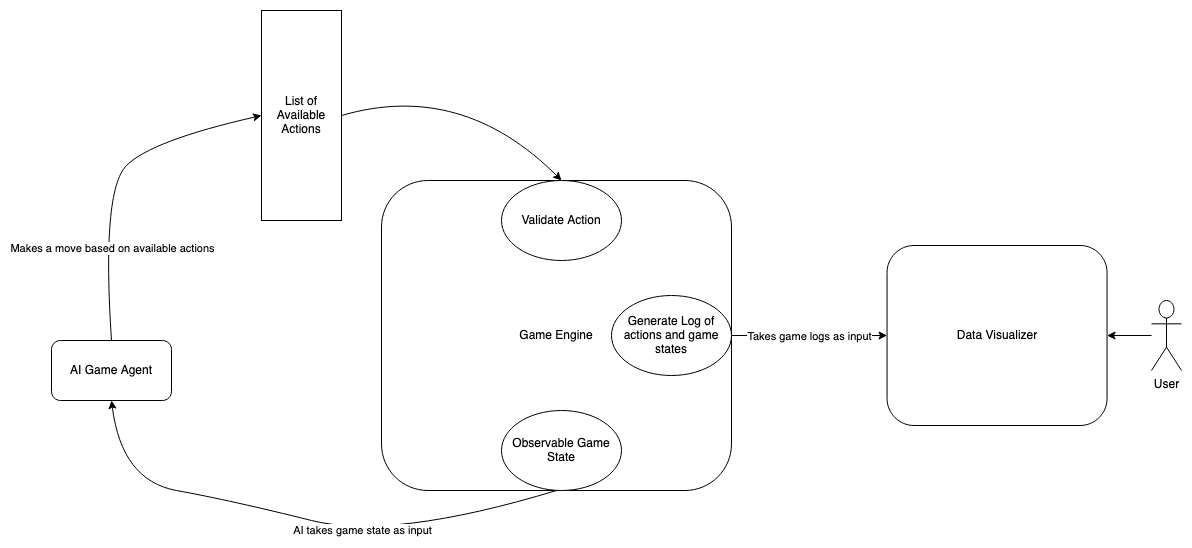
\includegraphics[width=1.0\textwidth]{SystemArchitecture.png}
\caption{System Context}
\label{Fig_SystemContext} 
\end{center}
\end{figure}

Inside the Game Engine, there will be a finite state machine that controls the main game loop. The finite state automata will be comprised of variables $<Q, \sum, \delta, q_{0}, F>$
\begin{itemize}
    \item $Q$ The set of states, for many systems will be almost infinite as there are many different states the game can get to. Tic-Tac-Toe for example has only 23 unique winning states, while a game like chess has almost infinitely many,
    \item $\sum$ The alphabet is a list of all possible moves from one state to another.
    \item $\delta:(Q,\sum) \xrightarrow[]{} Q$ The transition function that will take the current state and a possible move and output the new updated state.
    \item $q_0$ The starting state, for Tic-Tac-Toe would be an empty board, for Monopoly would be an empty board, and all players with their starting money.
    \item $F \subset Q$ The set of final states, this will be all the winning end game states for a player.
\end{itemize}
To simplify the set of states, only three will be used: start, finish and in progress. These will be denoted as $q_0, q_1, q_2$ respectively. 

\begin{figure}[h!]
\begin{center}
\begin{tikzpicture}[scale=0.2]
\tikzstyle{every node}+=[inner sep=0pt]
\draw [black] (10.6,-25.4) circle (3);
\draw (10.6,-25.4) node {$q0$};
\draw [black] (33,-25.4) circle (3);
\draw (33,-25.4) node {$q_1$};
\draw [black] (67.1,-25.4) circle (3);
\draw (67.1,-25.4) node {$q_2$};
\draw [black] (67.1,-25.4) circle (2.4);
\draw [black] (13.6,-25.4) -- (30,-25.4);
\fill [black] (30,-25.4) -- (29.2,-24.9) -- (29.2,-25.9);
\draw (21.8,-25.9) node [below] {$Begin\mbox{ }game$};
\draw [black] (36,-25.4) -- (64.1,-25.4);
\fill [black] (64.1,-25.4) -- (63.3,-24.9) -- (63.3,-25.9);
\draw (50.05,-25.9) node [below] {$Winning\mbox{ }move\mbox{ }is\mbox{ }played$};
\draw [black] (32.183,-22.525) arc (223.59229:-64.40771:2.25);
\draw (41.44,-16.94) node [above] {$Non-winning\mbox{ }valid\mbox{ }move\mbox{ }is\mbox{ }played$};
\fill [black] (34.78,-23) -- (35.71,-22.81) -- (35.02,-22.09);
\end{tikzpicture}
\caption{Finite State Machine for Game Loop}
\end{center}
\end{figure}
The game will continue until a winning move is played and loops after each non-winning move, and all non-valid moves are rejected. Based on the game non-valid moves could result in the game being forfeited and lost, for this simple example, the Game Engine will reject the AI Agent's move and wait for a valid one.\\ 

\textbf{User Responsibilities:}
\begin{itemize}
\item The Users will observe the data visualizer of game simulations. 
\end{itemize}


\textbf{System Responsibilities:}
\begin{itemize}
\item AI Agent: Receive input of a game state and output a decision. 
\item Available  Actions: List all available moves to the AI Agents (Not an entity itself and is a part of the Game Engine)
\item Game Engine: Receives inputs of decisions made by the AI Agents and updates its game state accordingly. Outputs a log file of the state and actions and the updated state back to the Game Agents.
\end{itemize}

\subsection{User Characteristics} \label{SecUserCharacteristics}
The intended users of the system will be AI research professors and game designers. These users will be observing the same output of the system, but analyzing it in a different way. The AI research professors will be using the output to analyze how different kinds of AI play a specific Game Engine. Meaning these users should have a deep understanding of AI, Neural Networks, Machine Learning, and other AI topics. The game designers will be using the output to check for any "over-powered" strategies or game-breaking rules, these users should have a deep understanding of the game rules and mechanics (For the specific Game Engine in use). For all users of the system should have an understanding of statistics up to Stats 3Y03 to read and understand the data output.

\subsection{System Constraints}
The main constraint of the system is it must be developed in Python as AI libraries are easiest to implement and highly supported, the Game Engine and all other components must be implemented in Python for simple compatibility and integration.

\subsection{Normal Operation \& Undesired Event Handling}
The system will have a main loop where all the operations will take place after the initialization until the win condition is reached, then the system will exit the loop and end the current game to provide data visualization. This initialization, main loop, and win condition can be modeled and think as a finite state machine. The process is explained in detail in Section 2.1 and visualized in Figure 2. In the event of an unexpected outcome, since the games to be simulated are extremely complex and each move changes the state of the game significantly, the simulation will start over instead of any error handling. This decision is justified by the fact that each simulation should take less than 5 minutes and no undesired event will have a harmful effect on the system. Thus, the cost of restarting is cheaper than any extensive undesired event handling since we would have to handle thousands of different scenarios if we were to decide to do undesired event handling rather than restarting that particular simulation.

\newpage
\section{Specific System Description}

This section first presents the problem description, which gives a high-level
view of the problem to be solved.  This is followed by definitions and assumptions.

\subsection{Problem Description} \label{Sec_pd}

Designing a game is not an easy task. Especially, if the game is not a software that can be updated with correction and balancing patches later on but a physical board game where an incorrect game design can result in significant financial and reputation costs. In complex games, there are multiple players, dozens of variables and actions that can be taken, and millions of possible scenarios that each decision and variable can cause. A good game should be a balanced one and should not contain any definitive way to win the game every single time to make it more competitive and fun. However, it is also humanly not possible to go through each scenario and balance all the variables to make sure there are no loopholes in the game. Our project is trying to create a process where game designers can see most of the scenarios and balance the game before even publishing by utilizing the power of computers.

\subsubsection{Goal Statements}

\noindent Given the inputs, the goal statements are:

\begin{itemize}

\item \textbf{Game Simulation}: The system must simulate good quality board games containing rules and strategies with no serious consequences of mistakes.

\item \textbf{AI Learning}:
The system must implement artificial intelligent players to play thousands of games efficiently to detect patterns and learn winning strategies.   

\item \textbf{Complex Problem Solving}:
The AI game players of the system must be able to analyze complex decision paths. Each different AI game player should have a different decision-making process.  

\item \textbf{Quality Data}:
The system must output readable and correct data to track and save decisions, game states, and patterns throughout the simulations, as well as compare simulations against each other to find winning strategies.

\item \textbf{Data Visualization Analysis}:
The system must provide a variety of charts to visualize the data for users.

\item \textbf{Live User Interface}:
The system should have a live user interface where users can view the game states in real-time and the actions that AI game players are making.


\end{itemize}

\subsection{Assumptions} \label{sec_assumpt}

\begin{itemize}

\item[A\refstepcounter{assumpnum}\theassumpnum \label{A_Reward_Function}:]
  The game to be analyzed will have a clear reward function that AI Agent can optimize its learning towards.
  
\item[A\refstepcounter{assumpnum}\theassumpnum \label{A_End_Condition}:]
  The game to be analyzed will have a clear win condition where the game ends.\\ 
  \textbf{Rationale}: It shouldn't be an open-ended, infinite game where the goal is to just increase your score but rather there should be a specific condition(s) that players are playing towards to win and end the game. Otherwise, AI agents won't be able to find the optimal actions to win the game but rather keep outputting sub-optimal decisions which will have little to no value for game design improvements.
  
\item[A\refstepcounter{assumpnum}\theassumpnum \label{A_Representable}:]
  The game to be analyzed will have concrete rules that a computer can represent and enforce.\\
  \textbf{Rationale}: If the game cannot be simulated digitally, then AI Agent cannot be trained on the game and the system wouldn't be able to generate any meaningful data to aid the game design process.

\end{itemize}

\section{Required Behaviour Overview}
Our project consists of three main subsystems– Game Engine, AI Agent, and a data visualizer. These subsystems will work together to help game developers find imbalances in the game mechanics as well as find strategies that result in higher-than-expected winning percentages. 
\\\\
\textbf{AI Agent} – An AI model trained to play the game at hand acting as one of the players of the game to give insights into the possible paths to be taken. It would analyze all possible paths that a player can take at any point in the game. It would take as input the game state information (current state and available moves for the player) and output the next move that the player will take. 
\\
\textbf{Game Engine} – Abstract representation of the actual game as software. Contains all the game rules, observation space (state of the game), and action space (possible moves and commands that a player can choose from). It is also responsible for validating input from the AI Agent and outputting the game state with the moves available for the player. 
\\
\textbf{Data Visualizer} - Read the Game Engine and AI Agent log, and provide diverse graphic representations of data and information of moves to game state transitions. It will take the output from both the AI Agent and Game Engine to provide a way for the user to decipher imbalances in the game.


\section{Functional Requirements}

\subsection{AI Agent's Functional Requirements}
\noindent

\begin{minipage}{\textwidth}
\renewcommand*{\arraystretch}{1.5}
\begin{tabular}{| p{\colAwidth} | p{\colBwidth}|}
\hline
\rowcolor[gray]{0.9}
\bf FR\refstepcounter{reqnum}\thereqnum \label{R_Input} & AI Agent should take the state as input.\\ 
\hline
\bf Rationale & AI Agent will not store the state information. Rather it will get it from the Game Engine as an input.\\
\hline
\bf Priority& High\\
\hline
\end{tabular}
\end{minipage}\\

\begin{minipage}{\textwidth}
\renewcommand*{\arraystretch}{1.5}
\begin{tabular}{| p{\colAwidth} | p{\colBwidth}|}
\hline
\rowcolor[gray]{0.9}
\bf FR\refstepcounter{reqnum}\thereqnum \label{R_Input} & AI Agent can be swapped with another AI Agent or a human player.\\ 
\hline
\bf Rationale & The project aims to provide a tool for all game designers to test their games. Every game will require a different AI model trained specifically on that game. Thus, AI Agent needs to be modular enough to swap with other AI Agents. \\
\hline
\bf Priority& Medium\\
\hline
\end{tabular}
\end{minipage}\\

\begin{minipage}{\textwidth}
\renewcommand*{\arraystretch}{1.5}
\begin{tabular}{| p{\colAwidth} | p{\colBwidth}|}
\hline
\rowcolor[gray]{0.9}
\bf FR\refstepcounter{reqnum}\thereqnum \label{R_Input} & AI Agent should be observable.\\ 
\hline
\bf Rationale & The decisions of the AI Agent should be recorded so that it can be reviewed by the game designer to guide the design of the board game.\\
\hline
\bf Priority& High\\
\hline
\end{tabular}
\end{minipage}\\

\begin{minipage}{\textwidth}
\renewcommand*{\arraystretch}{1.5}
\begin{tabular}{| p{\colAwidth} | p{\colBwidth}|}
\hline
\rowcolor[gray]{0.9}
\bf FR\refstepcounter{reqnum}\thereqnum \label{R_Input} & AI Agent should only output an action that is in the action space provided by the Game Engine.\\ 
\hline
\bf Rationale & By only selecting the actions in the action space provided by the Game Engine, errors will be reduced and the game can actually progress. \\
\hline
\bf Priority& High\\
\hline
\end{tabular}
\end{minipage}\\

\begin{minipage}{\textwidth}
\renewcommand*{\arraystretch}{1.5}
\begin{tabular}{| p{\colAwidth} | p{\colBwidth}|}
\hline
\rowcolor[gray]{0.9}
\bf FR\refstepcounter{reqnum}\thereqnum \label{R_Input} & AI Agent shall not see the state information that a human player cannot see.\\ 
\hline
\bf Rationale & In multiplayer games, there will be information specific to the user (e.g. hidden cards) which the AI Agent should not see to have the same level of visibility as a human player would have. \\
\hline
\bf Priority& High\\
\hline
\end{tabular}
\end{minipage}\\

\begin{minipage}{\textwidth}
\renewcommand*{\arraystretch}{1.5}
\begin{tabular}{| p{\colAwidth} | p{\colBwidth}|}
\hline
\rowcolor[gray]{0.9}
\bf FR\refstepcounter{reqnum}\thereqnum \label{R_Input} & AI Agent shall always respond with an action.\\ 
\hline
\bf Rationale & Even if there is no optimal move, AI Agent should output an action so that the game can progress.\\
\hline
\bf Priority& High\\
\hline
\end{tabular}
\end{minipage}\\

\subsection{Game Engine Functional Requirements}
\noindent

\begin{minipage}{\textwidth}
\renewcommand*{\arraystretch}{1.5}
\begin{tabular}{| p{\colAwidth} | p{\colBwidth}|}
\hline
\rowcolor[gray]{0.9}
\bf FR\refstepcounter{reqnum}\thereqnum \label{R_Output} & The Game Engine must validate the input from the AI Agent\\ 
\hline
\bf Rationale& One of the core functionality of our system is the interaction between the AI Agent and the Game Engine. The Game Engine must be responsible for validating the input (state) from the AI engine, to ensure the action taken is a valid action. \\
\hline
\bf Priority& High\\
\hline
\end{tabular}
\end{minipage}\\

\begin{minipage}{\textwidth}
\renewcommand*{\arraystretch}{1.5}
\begin{tabular}{| p{\colAwidth} | p{\colBwidth}|}
\hline
\rowcolor[gray]{0.9}
\bf FR\refstepcounter{reqnum}\thereqnum \label{R_Output} & The Game Engine must have an end/winning state to end the game.\\ 
\hline
\bf Rationale& A Game Engine's main role is to transition from the start state to the end state using the player's moves. The Game Engine must validate if a player(s) has reached the end state at any point of the gameplay.\\
\hline
\bf Priority& High\\
\hline
\end{tabular}
\end{minipage}\\

\begin{minipage}{\textwidth}
\renewcommand*{\arraystretch}{1.5}
\begin{tabular}{| p{\colAwidth} | p{\colBwidth}|}
\hline
\rowcolor[gray]{0.9}
\bf FR\refstepcounter{reqnum}\thereqnum \label{R_Output} & The Game Engine must output the current state of the game, if not in the end state.\\ 
\hline
\bf Rationale& As the AI Agent will be using the Game Engine's output to perform different moves, it is essential for the Game Engine to provide the current state of the game in order for the AI to make appropriate decisions.\\
\hline
\bf Priority& High\\
\hline
\end{tabular}
\end{minipage}\\

\begin{minipage}{\textwidth}
\renewcommand*{\arraystretch}{1.5}
\begin{tabular}{| p{\colAwidth} | p{\colBwidth}|}
\hline
\rowcolor[gray]{0.9}
\bf FR\refstepcounter{reqnum}\thereqnum \label{R_Output} & The Game Engine must follow all the playing and business rules of the game\\ 
\hline
\bf Rationale& It is necessary for the Game Engine to implement all the game rules such that it can validate moves and transition to the end state.\\
\hline
\bf Priority& High\\
\hline
\end{tabular}
\end{minipage}\\

\begin{minipage}{\textwidth}
\renewcommand*{\arraystretch}{1.5}
\begin{tabular}{| p{\colAwidth} | p{\colBwidth}|}
\hline
\rowcolor[gray]{0.9}
\bf FR\refstepcounter{reqnum}\thereqnum \label{R_Output} & The Game Engine must supply a list of game moves that an AI Agent can take.\\ 
\hline
\bf Rationale& It is necessary for the AI Agent to know what moves it can take. This move list does not ensure all moves are legal, only that they can be executed.\\
\hline
\bf Priority& High\\
\hline
\end{tabular}
\end{minipage}\\


\subsection{Game Data Visualization Analysis Requirement}
\noindent

\begin{minipage}{\textwidth}
\renewcommand*{\arraystretch}{1.5}
\begin{tabular}{| p{\colAwidth} | p{\colBwidth}|}
\hline
\rowcolor[gray]{0.9}
\bf FR\refstepcounter{reqnum}\thereqnum \label{R_Output} & The game system must generate a variety of data visualization charts\\ 
\hline
\bf Rationale &  The functionality of data visualization charts is to provide different graphic representations of data and information such as pie charts, bar graphs, and line charts to the users. It can efficiently show insights that may be missed in traditional reports and translates the data into a visual context that the users can understand easily.\\
\hline
\bf Priority& High\\
\hline
\end{tabular}
\end{minipage}\\


\begin{minipage}{\textwidth}
\renewcommand*{\arraystretch}{1.5}
\begin{tabular}{| p{\colAwidth} | p{\colBwidth}|}
\hline
\rowcolor[gray]{0.9}
\bf FR\refstepcounter{reqnum}\thereqnum \label{R_Output} & The game system must read data from the Game Engine and AI Agent logs. \\ 
\hline
\bf Rationale &  The functionality of reading data from the Game Engine and AI Agent allows the system to proceed with deeper data analysis.\\
\hline
\bf Priority& High\\
\hline
\end{tabular}
\end{minipage}\\

\begin{minipage}{\textwidth}
\renewcommand*{\arraystretch}{1.5}
\begin{tabular}{| p{\colAwidth} | p{\colBwidth}|}
\hline
\rowcolor[gray]{0.9}
\bf FR\refstepcounter{reqnum}\thereqnum \label{R_Output} & The game system must allow users to select different data points  \\ 
\hline
\bf Rationale &  It is necessary for users to select a variety of data points such as win percentages of different first moves taken, game state changes in different decision-making processes, and actions having the highest win rates. \\
\hline
\bf Priority& High\\
\hline
\end{tabular}
\end{minipage}\\



\begin{minipage}{\textwidth}
\renewcommand*{\arraystretch}{1.5}
\begin{tabular}{| p{\colAwidth} | p{\colBwidth}|}
\hline
\rowcolor[gray]{0.9}
\bf FR\refstepcounter{reqnum}\thereqnum \label{R_Output} & The game system compare data between different Game Engine and AI Agent logs.\\ 
\hline
\bf Rationale &  The functionality of data comparison evaluates and compares selected data points. For example, it can compare multiple AI players’ winning paths and output the most optimal option. \\
\hline
\bf Priority& Low\\
\hline
\end{tabular}
\end{minipage}\\


\newpage
\section{Nonfunctional Requirements}
This section will describe the non-functional requirements which will be the qualities the system has and why they are important and how they can be verified.

\subsection{Accuracy}
\begin{minipage}{\textwidth}
\renewcommand*{\arraystretch}{1.5}
\begin{tabular}{| p{\colAwidth} | p{\colBwidth}|}
\hline
\rowcolor[gray]{0.9}
\bf NFR\refstepcounter{nfrnum}\thenfrnum \label{NFR_Accuracy}: & The system, specifically the AI Agent should get more and more accurate after each simulation in choosing winning moves. After (Learning Benchmark) 1000 simulations an AI Agent should be able to win against its previous version. \\ 
\hline
\bf Rationale & Since some of the AI Agent's will be using reinforcement learning they must get more intelligent at playing the game after a duration of simulations. \\
\hline
\end{tabular}
\end{minipage}\\

\subsection{Usability}
\begin{minipage}{\textwidth}
\renewcommand*{\arraystretch}{1.5}
\begin{tabular}{| p{\colAwidth} | p{\colBwidth}|}
\hline
\rowcolor[gray]{0.9}
\bf NFR\refstepcounter{nfrnum}\thenfrnum \label{NFR_Accuracy}: & The system should be understood and navigable by the technical stakeholders (Dr .Mosser, Dr .Reinharz and Game Designers) after a (Understanding Benchmark) 30-minute explanation from the developers  \\ 
\hline
\bf Rationale & Usability of the system is not of high importance for the general public. The main users will be AI Research Professors and Game Designers, these two users will only be interacting with one part of the system, that is the data visualizer. Users familiar with data visualization software should have an easy time navigating and understanding the data. \\
\hline
\end{tabular}
\end{minipage}\\

\subsection{Modularity}
\begin{minipage}{\textwidth}
\renewcommand*{\arraystretch}{1.5}
\begin{tabular}{| p{\colAwidth} | p{\colBwidth}|}
\hline
\rowcolor[gray]{0.9}
\bf NFR\refstepcounter{nfrnum}\thenfrnum \label{NFR_Accuracy}: & The system should be modular enough to where additional AI Agents can be implemented in two days of development time. A Game Engine can be implemented in 7 days of development time.  \\ 
\hline
\bf Rationale & Modularity is a very important quality the system needs to have. All the components need to be easily swappable, that is AI Agents should be able to be changed with other implementations of AI, with minimal effort and the structure should support different Game Engines being integrated. \\
\hline
\end{tabular}
\end{minipage}\\

\subsection{Portability}
\begin{minipage}{\textwidth}
\renewcommand*{\arraystretch}{1.5}
\begin{tabular}{| p{\colAwidth} | p{\colBwidth}|}
\hline
\rowcolor[gray]{0.9}
\bf NFR\refstepcounter{nfrnum}\thenfrnum \label{NFR_Accuracy}: & The system should run on macOS Monterey and newer, Windows10 and newer, and on Aliance Canada's Computer Cluster. The simulation of the Game Engine with the AI Agent's must be able to run on each OS for them to be verified as working. \\ 
\hline
\bf Rationale & These operating systems will be used by the developers and the Aliance Canada's Computer Cluster will be used in case additional computing power is needed.\\
\hline
\end{tabular}
\end{minipage}\\

\subsection{Performance}
\begin{minipage}{\textwidth}
\renewcommand*{\arraystretch}{1.5}
\begin{tabular}{| p{\colAwidth} | p{\colBwidth}|}
\hline
\rowcolor[gray]{0.9}
\bf NFR\refstepcounter{nfrnum}\thenfrnum \label{NFR_Accuracy}: & The system should complete a single simulation in under (Speed Benchmark) 5 minutes. \\ 
\hline
\bf Rationale & If a simulation is taking too long it will slow down the learning of the AI Agents as well as take up resources from the developers' computers.\\
\hline
\end{tabular}
\end{minipage}\\

\subsection{Extensibility}
\begin{minipage}{\textwidth}
\renewcommand*{\arraystretch}{1.5}
\begin{tabular}{| p{\colAwidth} | p{\colBwidth}|}
\hline
\rowcolor[gray]{0.9}
\bf NFR\refstepcounter{nfrnum}\thenfrnum \label{NFR_Accuracy}: & The system should be able to be extended to include additional rules and mechanics in 2 days of development time. \\ 
\hline
\bf Rationale & With more complex games and games still in development rules and mechanics will be added iteratively rather than all at once.\\
\hline
\end{tabular}
\end{minipage}\\

\subsection{Look and Feel}
\begin{minipage}{\textwidth}
\renewcommand*{\arraystretch}{1.5}
\begin{tabular}{| p{\colAwidth} | p{\colBwidth}|}
\hline
\rowcolor[gray]{0.9}
\bf NFR\refstepcounter{nfrnum}\thenfrnum \label{NFR_Accuracy}: & The system specifically the Data Visualizer should clearly indicate data using different colours, lines and shapes. Should appeal to more than 75\% (Look Feel Benchmark) of game designers  \\ 
\hline
\bf Rationale & With a clear and clean look the data will be easier to visualize.\\
\hline
\end{tabular}
\end{minipage}\\
\subsection{Security}
N/A
\subsection{Cultural and Political}
N/A
\subsection{Legal}
N/A

\section{Phase-In Plan}
All requirements with \textit{High} priority must be implemented prior to the Revision 0 demonstration (February 6-17, 2023) as they represent the core functionality of our system.
\\All requirements with \textit{Medium} priority will be implemented before the Revision 1 demonstration (March 20-31, 2023). 
\\All requirements with \textit{Low} priority will be added after all \textit{High} and \textit{Medium} requirements are implemented, time permitting.


\newpage
\section{Likelihood of Changes for Functional Requirements}    


\begin{table}[H]
\begin{tabular}{|l|p{0.20\textwidth}|p{0.34\textwidth}|p{0.20\textwidth}|l}
\cline{1-4}
\centering{\textbf{Requirement}} & \centering{\textbf{Likelihood of Change}} & \centering{\textbf{Rationale}}                                                                               & \centering{\textbf{Ways to Change}}                            &  \\ \cline{1-4}
\textbf{FR1}                                & Very Unlikely                                      & Core implementation aspect                                                                                            & N/A                                                                     &  \\ \cline{1-4}
\textbf{FR2}                                & Very Unlikely                                      & Core implementation aspect                                                                                            & N/A                                                                     &  \\ \cline{1-4}
\textbf{FR3}                                & Very Unlikely                                      & Core implementation aspect                                                                                            & N/A                                                                     &  \\ \cline{1-4}
\textbf{FR4}                                & Very Unlikely                                      & Must produce valid actions within the space or the system could loop indefinitely                                     & N/A                                                                     &  \\ \cline{1-4}
\textbf{FR5}                                & Very Unlikely                                      & AI Agent should not have an advantage over a human player                                                             & N/A                                                                     &  \\ \cline{1-4}
\textbf{FR6}                                & Very Unlikely                                      & Must produce an action or the system cannot continue function                                                         & N/A                                                                     &  \\ \cline{1-4}
\textbf{FR7}                                & Very Unlikely                                      & Core implementation aspect                                                                                            & N/A                                                                     &  \\ \cline{1-4}
\textbf{FR8}                                & Very Unlikely                                      & Core implementation aspect                                                                                            & N/A                                                                     &  \\ \cline{1-4}
\textbf{FR9}                                & Very Unlikely                                      & Important to visualize the state game for data analysis and allows for a human player to understand the state of game & N/A                                                                     &  \\ \cline{1-4}
\textbf{FR10}                               & Very Unlikely                                      & Core implementation aspect                                                                                            & N/A                                                                     &  \\ \cline{1-4}
\textbf{FR11}                               & Very Unlikely                                      & Allows for the AI Agent to generate a valid action to prevent invalid actions                                         & N/A                                                                     &  \\ \cline{1-4}
\textbf{FR12}                               & Unlikely                                           & May produce only a specific visualization data charts                                                                 & Produce only specific data visualization charts                         &  \\ \cline{1-4}
\textbf{FR13}                               & Very Unlikely                                      & Required for the stakeholder to understand the data                                                                   & N/A                                                                     &  \\ \cline{1-4}
\textbf{FR14}                               & Unlikely                                           & Subject to time constraints, is not required in the minimal viable product but highly valued for the stakeholder                                            & Requirement is removed and function is not implemented in final product &  \\ \cline{1-4}
\textbf{FR15}                               & Likely                                           & Subject to time constraints, is not required in the minimal viable product                                            & Requirement is removed and function is not implemented in final product &  \\ \cline{1-4}
\end{tabular}
\end{table}

<<<<<<< HEAD
\newpage
=======
\plt{This section is not for test cases or techniques for verification and
  validation.  Those topics will be addressed in the Verification and Validation
  plan.}

\section{Requirements}

\plt{The requirements refine the goal statement.  They will make heavy use of
  references to the instance models.}

This section provides the functional requirements, the business tasks that the
software is expected to complete, and the nonfunctional requirements, the
qualities that the software is expected to exhibit.

\subsection{Functional Requirements}

\noindent \begin{itemize}

\item[R\refstepcounter{reqnum}\thereqnum] AI agent should take the state as input.

\item[R\refstepcounter{reqnum}\thereqnum] Game Engine should supply/output game state.

\item[R\refstepcounter{reqnum}\thereqnum] Game Engine should only accept legal actions/commands. %should we also have another requirement: AI should only output legal action/command

\item[R\refstepcounter{reqnum}\thereqnum] 

\item[R\refstepcounter{reqnum}\thereqnum]

\item[R\refstepcounter{reqnum}\thereqnum \label{R_Inputs}:] \plt{Requirements
    for the inputs that are supplied by the user.  This information has to be
    explicit.}

\item[R\refstepcounter{reqnum}\thereqnum \label{R_OutputInputs}:] \plt{It isn't
    always required, but often echoing the inputs as part of the output is a
    good idea.}

\item[R\refstepcounter{reqnum}\thereqnum \label{R_Calculate}:] \plt{Calculation
    related requirements.}

\item[R\refstepcounter{reqnum}\thereqnum \label{R_VerifyOutput}:]
  \plt{Verification related requirements.}

\item[R\refstepcounter{reqnum}\thereqnum \label{R_Output}:] \plt{Output related
    requirements.}

\end{itemize}

\plt{Every IM should map to at least one requirement, but not every requirement
  has to map to a corresponding IM.}

\subsection{Nonfunctional Requirements}

\plt{List your nonfunctional requirements.  You may consider using a fit
  criterion to make them verifiable.}
\plt{The goal is for the nonfunctional requirements to be unambiguous, abstract
  and verifiable.  This isn't easy to show succinctly, so a good strategy may be
to give a ``high level'' view of the requirement, but allow for the details to
be covered in the Verification and Validation document.}
\plt{An absolute requirement on a quality of the system is rarely needed.  For
  instance, an accuracy of 0.0101 \% is likely fine, even if the requirement is
  for 0.01 \% accuracy.  Therefore, the emphasis will often be more on
  describing now well the quality is achieved, through experimentation, and
  possibly theory, rather than meeting some bar that was defined a priori.}
\plt{You do not need an entry for correctness in your NFRs.  The purpose of the
  SRS is to record the requirements that need to be satisfied for correctness.
  Any statement of correctness would just be redundant. Rather than discuss
  correctness, you can characterize how far away from the correct (true)
  solution you are allowed to be.  This is discussed under accuracy.}

\noindent \begin{itemize}

\item[NFR\refstepcounter{nfrnum}\thenfrnum \label{NFR_Accuracy}:]
  \textbf{Accuracy} \plt{Characterize the accuracy by giving the context/use for
    the software.  Maybe something like, ``The accuracy of the computed
    solutions should meet the level needed for $<$engineering or scientific
    application$>$.  The level of accuracy achieved by \progname{} shall be
    described following the procedure given in Section~X of the Verification and
    Validation Plan.''  A link to the VnV plan would be a nice extra.}

\item[NFR\refstepcounter{nfrnum}\thenfrnum \label{NFR_Usability}:] \textbf{Usability}
  \plt{Characterize the usability by giving the context/use for the software.
    You should likely reference the user characteristics section.  The level of
    usability achieved by the software shall be described following the
    procedure given in Section~X of the Verification and Validation Plan.  A
    link to the VnV plan would be a nice extra.}

\item[NFR\refstepcounter{nfrnum}\thenfrnum \label{NFR_Maintainability}:]
  \textbf{Maintainability} \plt{The effort required to make any of the likely
    changes listed for \progname{} should be less than FRACTION of the original
    development time.  FRACTION is then a symbolic constant that can be defined
    at the end of the report.}

\item[NFR\refstepcounter{nfrnum}\thenfrnum \label{NFR_Portability}:]
  \textbf{Portability} \plt{This NFR is easier to write than the others.  The
    systems that \progname{} should run on should be listed here.  When possible
    the specific versions of the potential operating environments should be
    given.  To make the NFR verifiable a statement could be made that the tests
    from a given section of the VnV plan can be successfully run on all of the
    possible operating environments.}

\item Other NFRs that might be discussed include verifiability,
  understandability and reusability.

\end{itemize}

\section{Likely Changes}    

\noindent \begin{itemize}

\item[LC\refstepcounter{lcnum}\thelcnum\label{LC_meaningfulLabel}:] \plt{Give
    the likely changes, with a reference to the related assumption (aref), as appropriate.}

\end{itemize}

\section{Unlikely Changes}    

\noindent \begin{itemize}

\item[LC\refstepcounter{lcnum}\thelcnum\label{LC_meaningfulLabel}:] \plt{Give
    the unlikely changes.  The design can assume that the changes listed will
    not occur.}

\end{itemize}

>>>>>>> 8588ba313814298fab11ccbd69ba232389ed6cd6
\section{Traceability Matrices and Graphs}
The table below shows the traceability matrix in how functional requirements depend on each other as well as depend on non-functional requirements and assumptions.
\begin{table}[h!]
\resizebox{17cm}{!} 
{
\begin{tabular}{|l|l|l|l|l|l|l|l|l|l|l|l|l|l|l|l|l|l|l|l|l|l|l|l|l|l|}
\hline
\textbf{ITEM} &
  \textbf{FR1} &
  \textbf{FR2} &
  \textbf{FR3} &
  \textbf{FR4} &
  \textbf{FR5} &
  \textbf{FR6} &
  \textbf{FR7} &
  \textbf{FR8} &
  \textbf{FR9} &
  \textbf{FR10} &
  \textbf{FR11} &
  \textbf{FR12} &
  \textbf{FR13} &
  \textbf{FR14} &
  \textbf{FR15} &
  \textbf{NFR1} &
  \textbf{NFR2} &
  \textbf{NFR3} &
  \textbf{NFR4} &
  \textbf{NFR5} &
  \textbf{NFR6} &
  \textbf{NFR7} &
  \textbf{A1} &
  \textbf{A2} &
  \textbf{A3} \\ \hline
\textbf{FR1}  &   &   &   &   &   &   &   &   & X &   &   &   &   &   &   & X &   & X &  & X & X &   &   &   &   \\ \hline
\textbf{FR2}  &   &   &   &   & X &   & X &   &   &   & X &   & X &   & X & X &   & X &  & X & X &   &   &   &   \\ \hline
\textbf{FR3}  &   &   &   &   &   &   &   &   &   &   &   &   & X &   & X &   &   &   &  &   &   &   &   &   &   \\ \hline
\textbf{FR4}  &   &   &   &   &   &   &   &   &   &   & X &   &   &   &   & X &   & X &  & X & X &   &   &   & X \\ \hline
\textbf{FR5}  &   & X &   &   &   &   &   &   &   &   &   &   &   &   &   &   &   &   &  &   &   &   &   &   &   \\ \hline
\textbf{FR6}  &   &   &   &   &   &   & X &   &   & X &   &   &   &   &   & X &   &   &  & X &   &   & X &   &   \\ \hline
\textbf{FR7}  &   & X &   &   &   & X &   &   &   &   &   &   &   &   &   &   &   &   &  &   &   &   &   &   & X \\ \hline
\textbf{FR8}  &   &   &   &   &   &   &   &   &   &   &   &   &   &   &   & X &   &   &  & X &   &   & X & X &   \\ \hline
\textbf{FR9}  & X &   &   &   &   &   &   &   &   &   &   &   &   &   &   &   &   &   &  & X &   &   &   &   &   \\ \hline
\textbf{FR10} &   &   &   &   &   & X &   &   &   &   &   &   &   &   &   &   &   &   &  &   &   &   &   &   & X \\ \hline
\textbf{FR11} &   & X &   & X &   &   &   &   &   &   &   &   &   &   &   & X &   &   &  &   &   &   &   &   &   \\ \hline
\textbf{FR12} &   &   &   &   &   &   &   &   &   &   &   &   &   &   &   &   & X &   &  &   &   & X &   &   &   \\ \hline
\textbf{FR13} &   & X & X &   &   &   &   &   &   &   &   &   &   &   &   &   &   &   &  &   &   &   &   &   &   \\ \hline
\textbf{FR14} &   &   &   &   &   &   &   &   &   &   &   &   &   &   &   &   & X &   &  &   &   & X &   &   &   \\ \hline
\textbf{FR15} &   & X & X &   &   &   &   &   &   &   &   &   &   &   &   &   & X &   &  &   &   & X &   &   &   \\ \hline
\textbf{NFR1} & X & X &   & X &   & X &   & X &   &   & X &   &   &   &   &   &   &   &  &   &   &   &   &   &   \\ \hline
\textbf{NFR2} &   &   & X &   &   &   &   &   &   &   &   & X &   & X & X &   &   &   &  &   &   &   &   &   &   \\ \hline
\textbf{NFR3} & X & X &   & X &   &   &   &   &   &   &   &   &   &   &   &   &   &   &  &   &   &   &   &   &   \\ \hline
\textbf{NFR4} &   &   &   &   &   &   &   &   &   &   &   &   &   &   &   &   &   &   &  &   &   &   &   &   &   \\ \hline
\textbf{NFR5} & X & X &   & X &   & X &   & X & X &   &   &   &   &   &   &   &   &   &  &   &   &   &   &   &   \\ \hline
\textbf{NFR6} & X & X &   & X &   &   &   &   &   &   &   &   &   &   &   &   &   &   &  &   &   &   &   &   &   \\ \hline
\textbf{NFR7} &   &   &   &   &   &   &   &   &   &   &   & X &   & X & X &   &   &   &  &   &   &   &   &   &   \\ \hline
\textbf{A1}   &   &   &   &   &   & X &   & X &   &   &   &   &   &   &   &   &   &   &  &   &   &   &   &   &   \\ \hline
\textbf{A2}   &   &   &   &   &   &   &   & X & X &   &   &   &   &   &   &   &   &   &  &   &   &   &   &   &   \\ \hline
\textbf{A3}   &   &   &   & X &   &   & X &   &   & X &   &   &   &   &   &   &   &   &  &   &   &   &   &   &   \\ \hline
\end{tabular}
}
\end{table}


\section{Impact Analysis}

This system will impact society as a stakeholder through the means of cultural factors as it is dealing with managing the quality of entertainment or specifically, the quality of board games. Completing this system will provide board game designers and game designers as a whole with a different and quicker means of balancing their turn-based games with AI. Being able to simulate many games in parallel to find unbalanced strategies in their games will allow them to produce these higher quality games for society to enjoy. In terms of health, safety, and other factors, this system will have a minimal impact.

\section{Values of Constants}
\begin{itemize}
\item Learning Benchmark: 1000 simulations
\item Understanding Benchmark: 30 minutes
\item Speed Benchmark: 5 minutes
\item Look and Feel Benchmark: 75\%

\end{itemize}

\section{Reflection Appendix}
\subsection{Game mechanics and rules}
\\
Assigned Team Members: \textit{All}
\\
All team members will be required to thoroughly understand the game rules for all the games we will be working on. This knowledge and expertise will be acquired through playing the game, reading game rule books, and any online resources that explain the rules of the games.
\\\\
Every team member will be using all the discussed methods to gain the expertise in this domain as it is easy for everyone to understand the game rules by playing the game and then reading the game rule books to further enhance their knowledge.

\\
\subsection{AI Agent}
\\
Assigned Team Members: \textit{Jeffrey and Jonah}
\\
Learning how to develop and implement an AI Agent will require the knowledge and learning of specific AI APIs and libraries. The skills acquired from learning how these APIs and libraries work will allow the team to create feasible enough agents to generate viable moves for the Game Engine to accept. The team members assigned for developing the AI Agents will begin with reinforcement learning libraries, Gym, PettingZoo, and SIMPLE, as a starting point to see if any viable AI Agents can be implemented with them and see if the team can further progress to other libraries. The team members were chosen for this topic for their previous experience in the machine learning course, COMPSCI 4ML3: Introduction to Machine Learning, and it should assist them in having to learn these libraries.
\\
Approaches to learn these libraries will involve dealing with tutorials, working with the starter code, and reading through the documentation.
\\\\
Jonah will use a combination of tutorials and documentation as he is able to understand better through tutorials and then he will be able to continue enforcing his knowledge further with the documentation given for the APIs and libraries.
\\\\
Jeffrey will begin by working on the starter code and continue will changing parameters in the starter code to see what output results as a consequence. Additionally, the use of the documentation will help change the starter code successfully. The reason for choosing this approach is because he particularly enjoys implementing first and then debugging towards the desired result afterward.
\subsection{Game Engine}
\\
Assigned Team Members: \textit{Michael and Hargun}
\\
Knowledge of Game Engine development and object-oriented programming is expected for this subsystem. The group members responsible for this subsystem will need to gain an understanding of how a Game Engine works and the level of abstraction it requires for it to be compatible with the other subsystems. The team members are also required to have experience with Python and have the thorough understanding principles of object-oriented programming. It is expected team members have a basic understanding of all libraries and frameworks that are used during the development of this subsystem. 
\\Knowledge and expertise will be gained through online tutorials, online articles, documentations of libraries/frameworks that are used, and through our supervisors.
\\\\Hargun will be using online tutorials and documentation to gain expertise in this domain area as it he finds it easier to learn from practical examples and then apply it to the desired problem.
\\\\Michael will be using online articles, documentation and our supervisors' expertise to gain knowledge in this domain area. Michael likes to research thoroughly before trying to solve a problem which is why it is beneficial for him to use these methods.


\subsection{Data Visualization Analysis}
\\
Assigned Team Members: \textit{Tianzheng}
\\
Data Visualization Analysis will require developers to understand users' expected data points, graphic representations, and what types of data need to compare. The group members are required to have sufficient knowledge of python data science libraries such as Matplotlib, Seaborn, NumPy, and pandas to create informative graphics and present accurate information to the users efficiently. 
\\\\
Tianzheng will be using online tutorials and documentation to gain expertise in data visualization and data analysis so as to find the most effective way to analyze the logs from the Game Engine and AI Agent. 
\newpage

\bibliographystyle {plainnat}
\bibliography {../../refs/References}

\end{document}